\documentclass[letterpaper]{article}
\usepackage{natbib,alife13}

\title{Aracna: An Open-Source Quadruped Platform for Evolutionary Robotics}
\author{Sara Lohmann, Eric Gold, Jeremy Blum, Jason Yosinski \and Hod Lipson \\
\mbox{}\\
Cornell University, 239 Upson Hall, Ithaca, NY 14853 \\
\texttt{sml253@cornell.edu}}





\begin{document}
\maketitle

\begin{abstract}
We report on a new open-source quadruped robotic platform, Aracna,
developed at Cornell's Creative Machines Lab for robotics
experiments. The robot comprises four legs with two joints each for a
total of eight kinematic degrees of freedom. Four-bar linkage
mechanisms in each leg drive the pitch of the knee joint and the hip
joint remotely, allowing the motors to remain in the robot center,
which reduces the inertia of each leg. Due to these non-conventional
kinematics, the robot requires non-intuitive movements for locomotion
and provides an interesting challenge for gait learning
algorithms. Aracna is a low-cost, accessible robotic platform for
testing in the real world.
\end{abstract}



\section{Introduction}

We address the need for a low-cost platform with non-intuitive walking
kinematics to explore evolutionary robotics. Aracna is the third
evolutionary learning quadruped robot developed by the Creative
Machines Lab \citep{HL, JY}. A common feature among the quadruped
robots is two actuators that drive the flexion/extension of a knee and
hip joint around parallel axes in each leg. The original Creative
Machines Lab quadruped robot favored starfish-like movements
\citep{HL}. The second quadruped robot --- QuadraTot ---
developed spider-like movements but was found to be limited by its
weight \citep{JY}. When creating the Aracna, we designed the hardware to
complement fast spider-like movements.

\begin{figure}[t]
\begin{center}
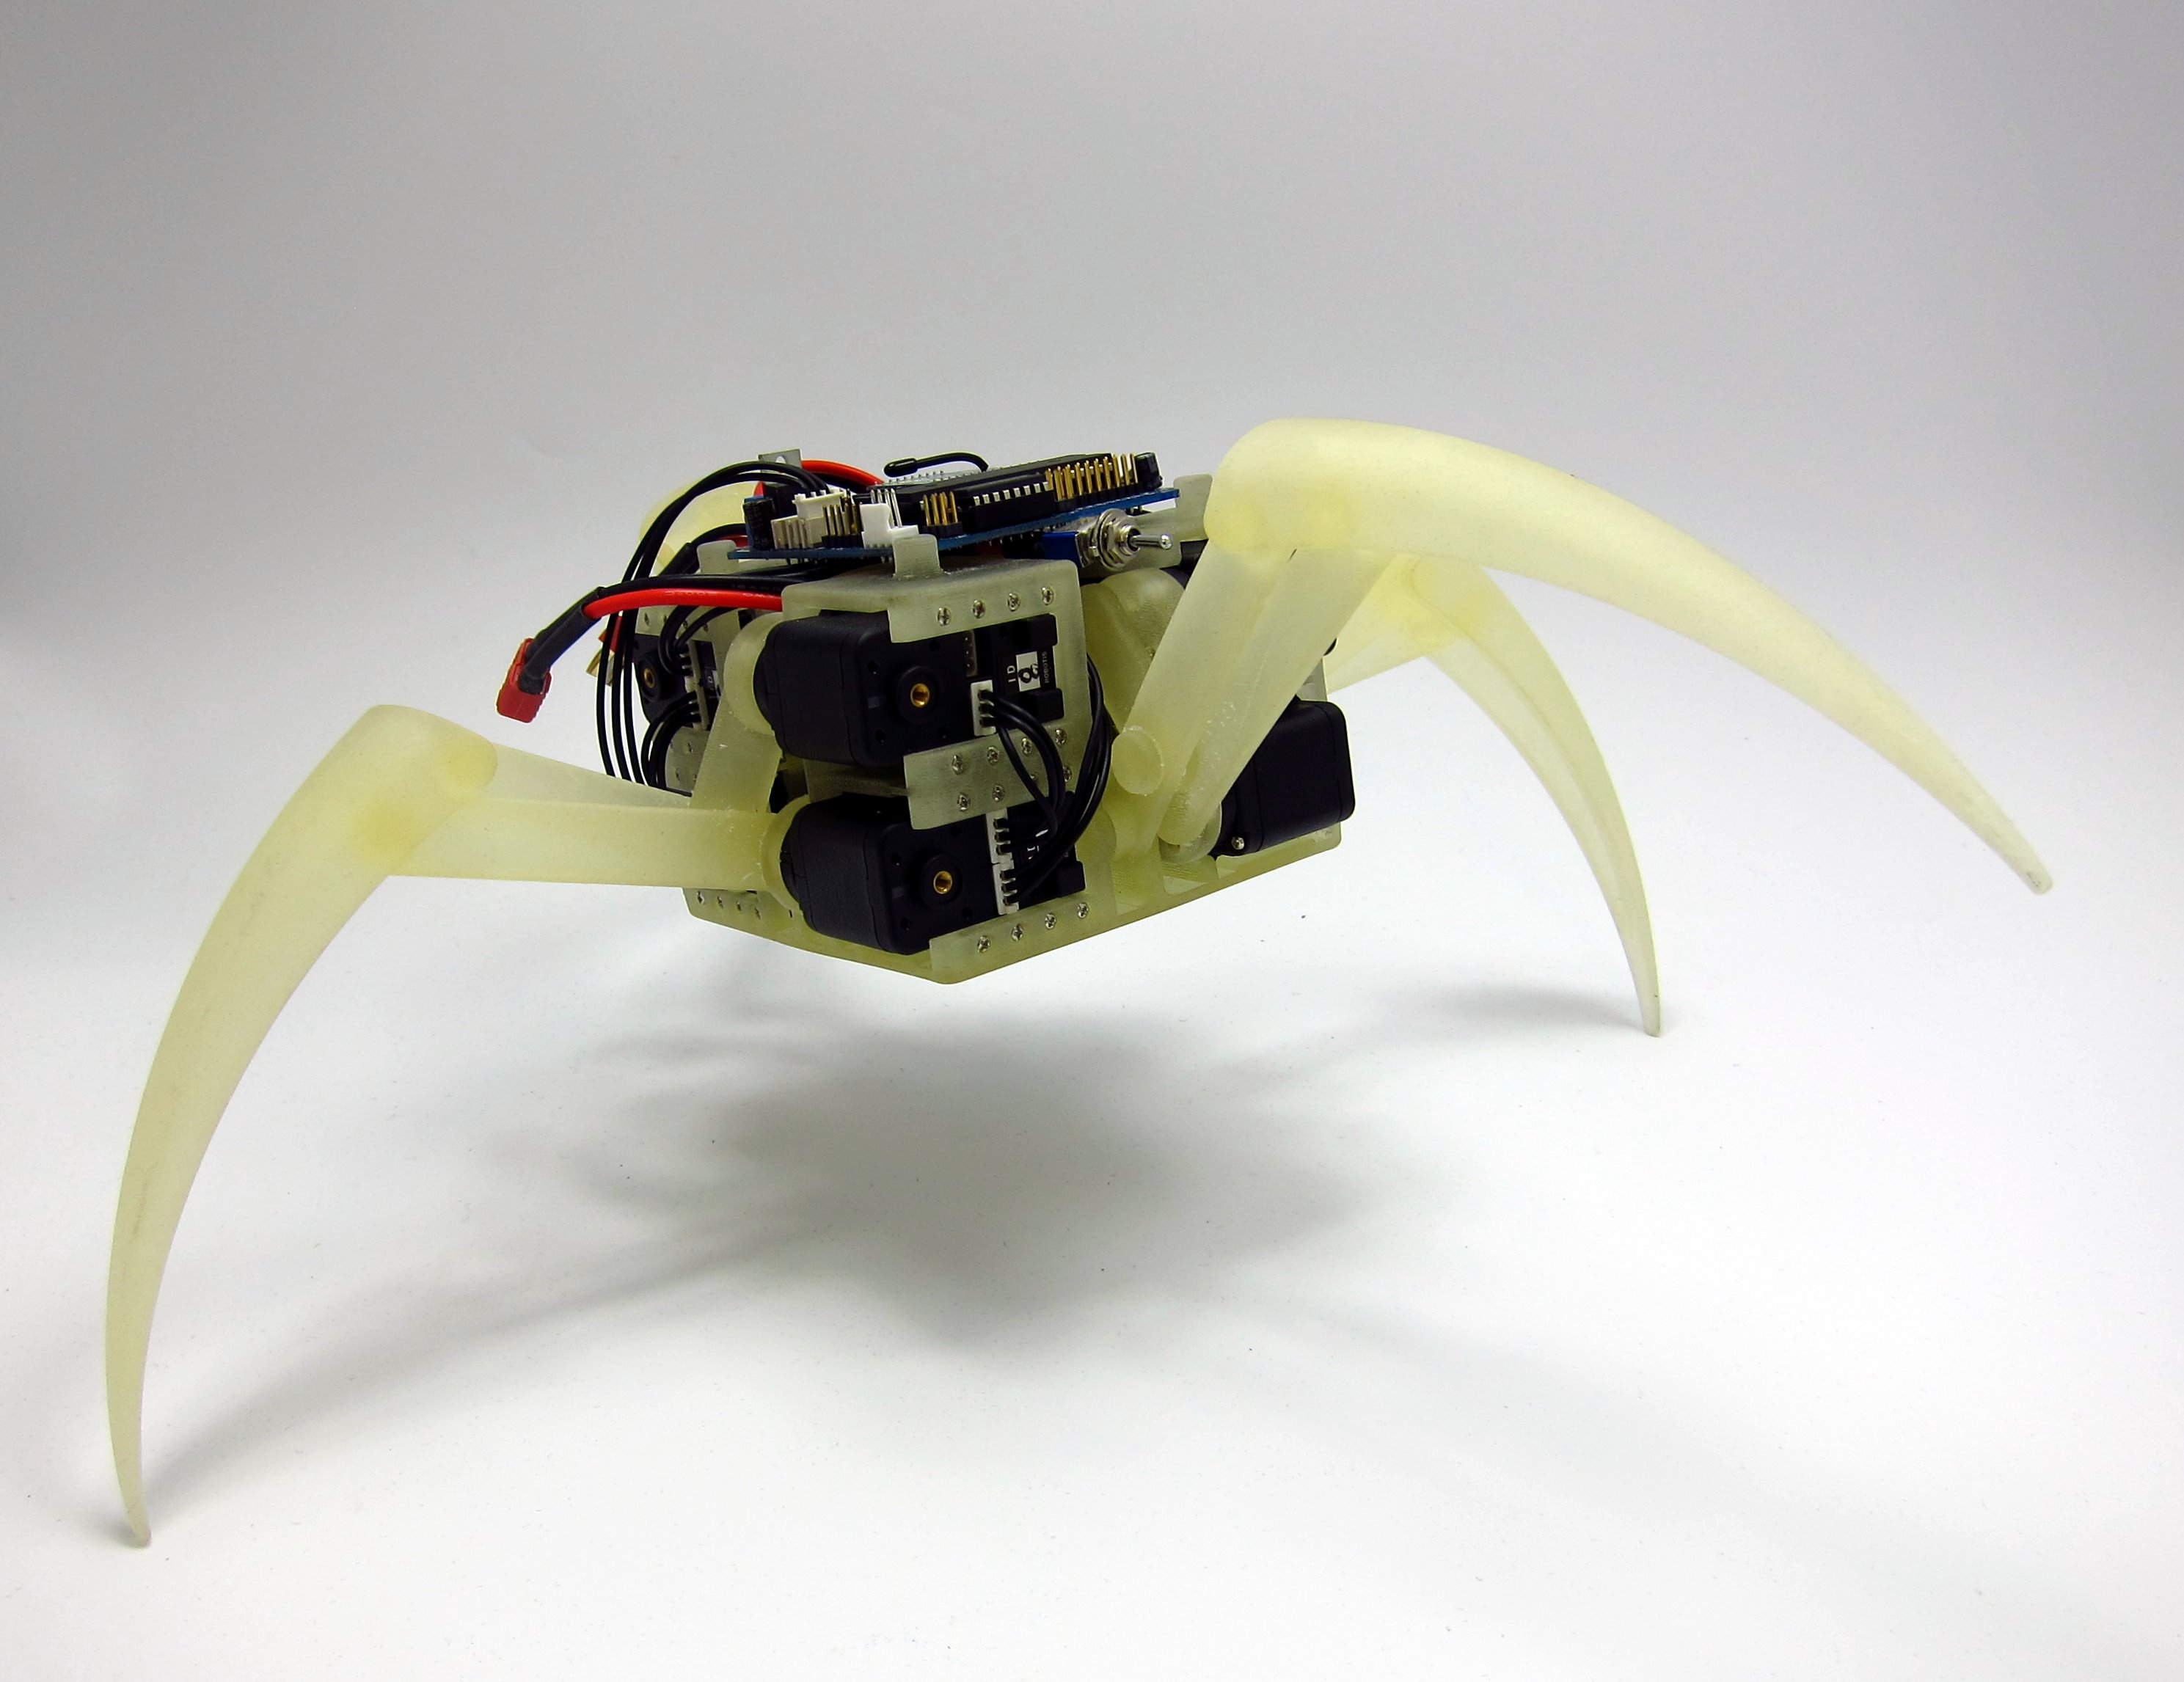
\includegraphics[width=.45\textwidth]{fig1.jpg}
\caption{Aracna: an open-sourced quadruped robot platform. All
  instructions and downloads are publicly available at
  http://creativemachines.cornell.edu/aracna .}
\label{fig1}
\end{center}
\end{figure}



\section{Hardware}

\begin{figure}[t]
\begin{center}
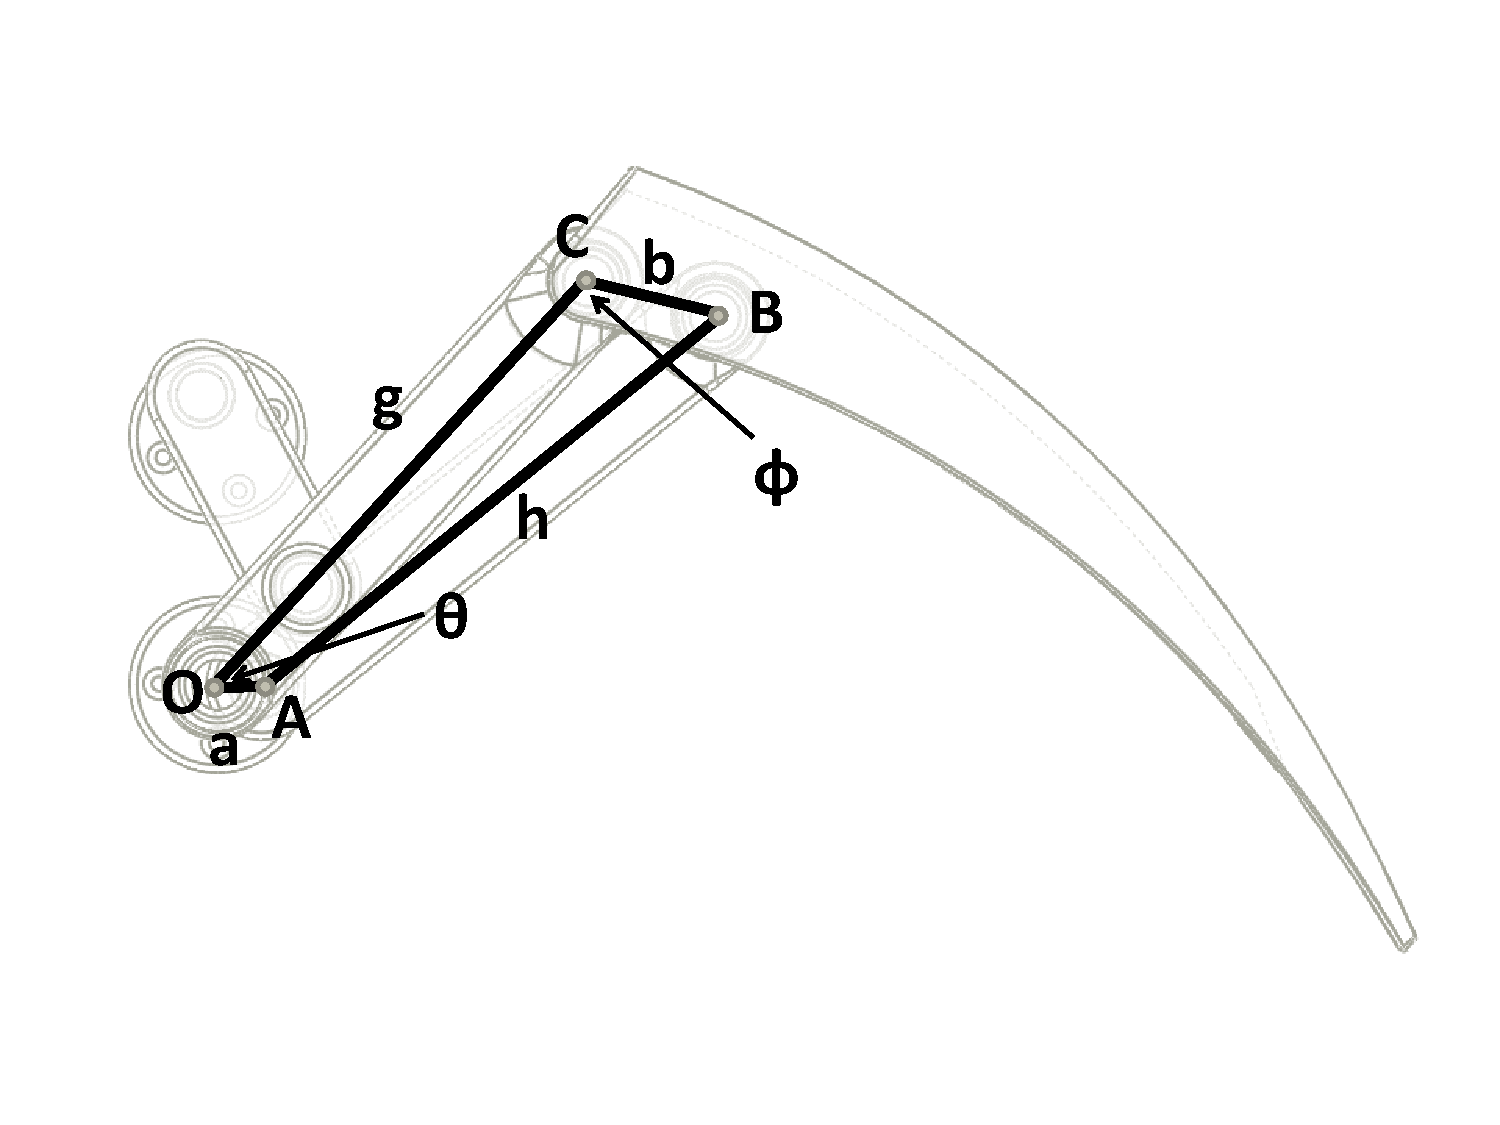
\includegraphics[width=.23\textwidth]{fig3.pdf}
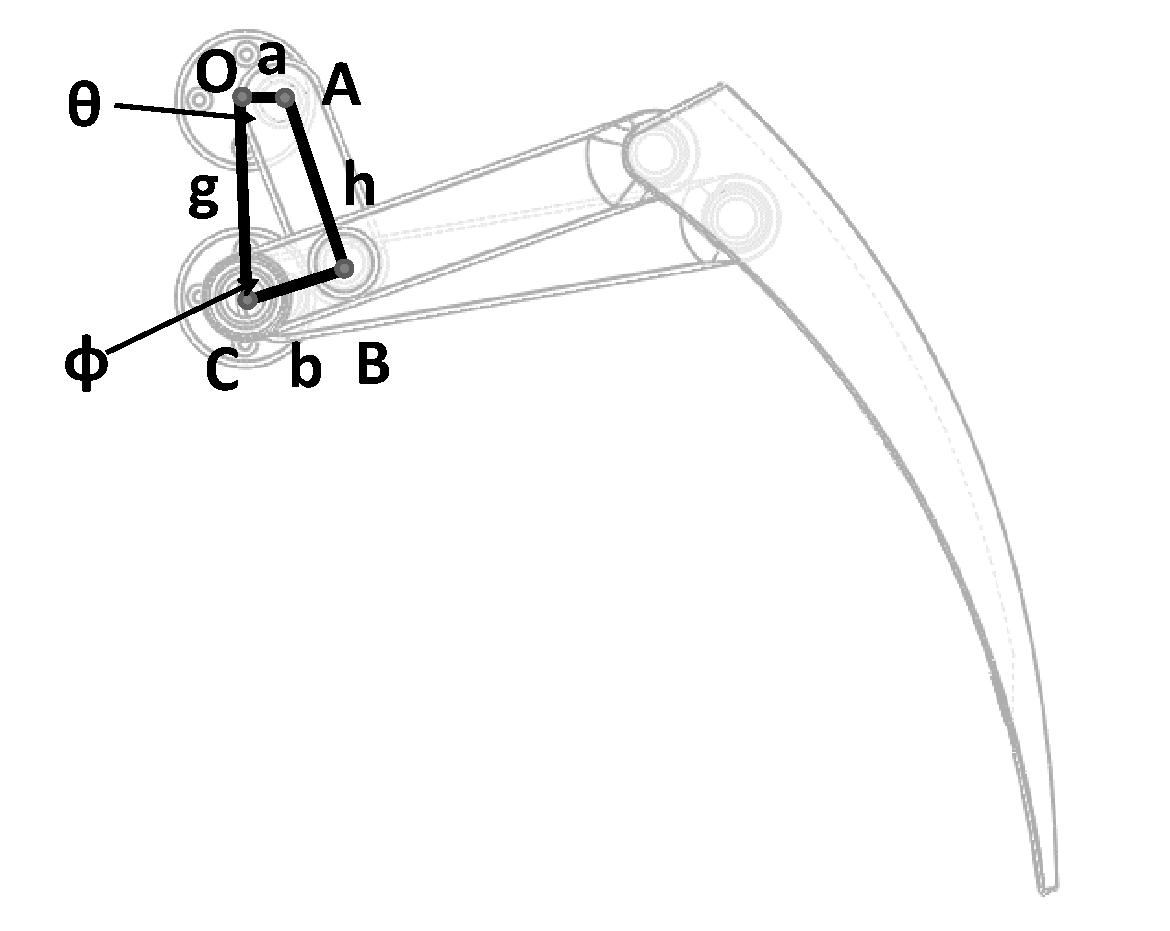
\includegraphics[width=.23\textwidth]{fig4.pdf}
\caption{Crank-rocker four-bar linkage controlling flexion/extension of
  the knee and hip joints. In both cases above, the input crank (link
  OA) is actuated by a servo, the rocker is the leg (link CB), and the
  fixed link is OC.}
\label{fig3}
\end{center}
\end{figure}

%\begin{figure}[t]
%\begin{center}
%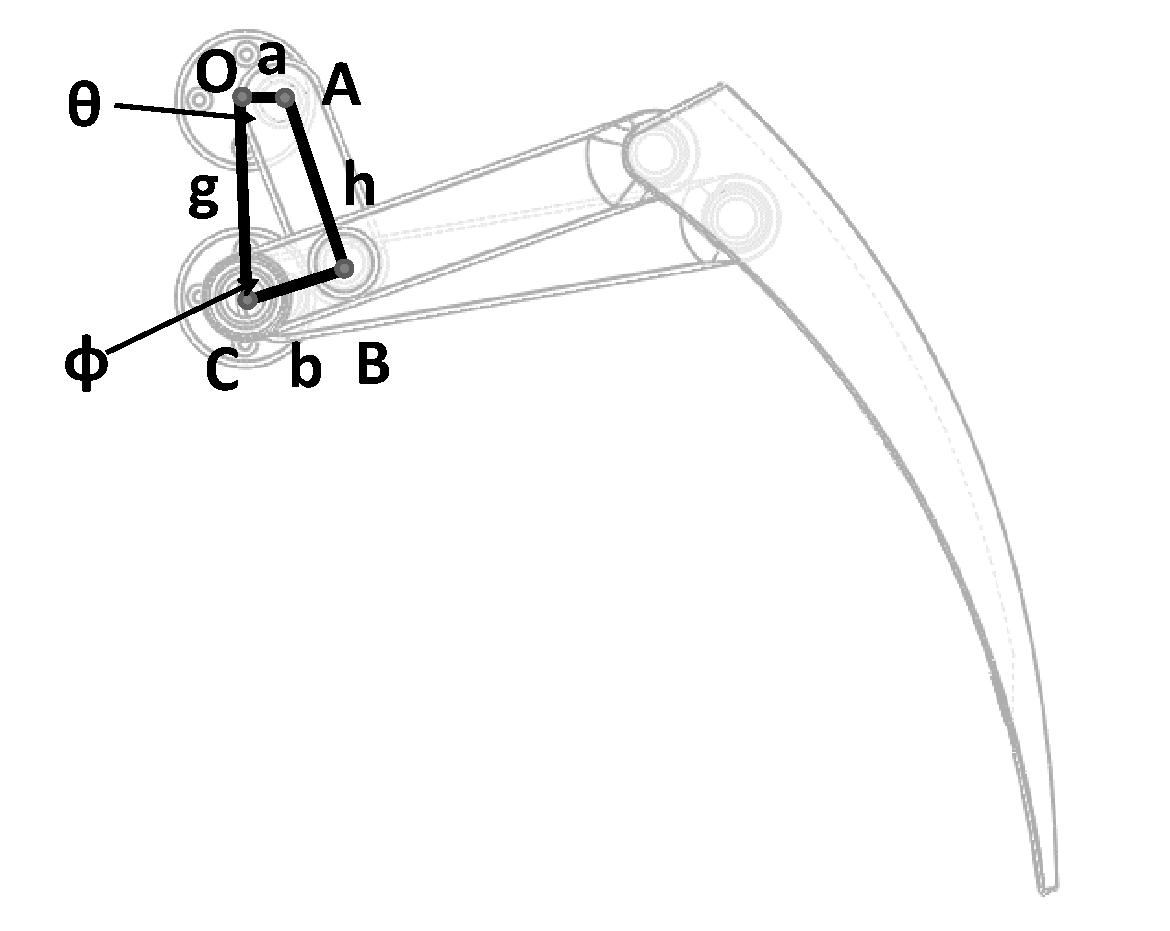
\includegraphics[width=2.25in,angle=0]{fig4.pdf}
%\caption{Crank-rocker four-bar linkage controlling flexion/extension of the hip joint.}
%\label{fig4}
%\end{center}
%\end{figure}

The hardware of Aracna evolved from the previous Creative Machines Lab
quadruped robots. We kept the same two degree of freedom pitch joint
scheme but decreased the weight and constrained the movement of the
joints toward the goal of creating faster spider-like movement. To
prevent starfish-like movement, the legs were constrained. We designed
the robot with two four-bar mechanisms to drive the joints in each
leg. With a four-bar mechanism in place, the leg moves at a fraction
of the output angle of the actuator, giving the motor a relatively
larger mechanical advantage over the position of each leg.
Figure~\ref{fig3} shows the crank-rocker system, where the input crank
is actuated by a servo and the rocker is the leg. In this
configuration, we keep the servo motors contained in the center of the
robot, reducing both the inertia and mass of each leg. The four-bar
mechanisms satisfied the design goal of making a robot that had
non-traditional movements.  To make the robot
accessible as an open-source platform, it was designed to be 3D
printed. The 3D print files and CAD files can be accessed by the
public to be printed and, if desired, modified.

The robot is designed to be lightweight, because previous similar
robots may have been too heavy and underpowered to generate
interesting gaits. We use a single LiPo 11.1V battery to
power 8 Dynamixel AX-18 servo motors and an ArbotiX
microcontroller. The main processing occurs on an external computer,
which allows the robot to have cheaper and lighter components
on-board. The space in the center of the body houses the
battery to reduce material weight and cost. Aracna weighs 1.03 kg.
% 1034g

\begin{figure}[t]
\begin{center}
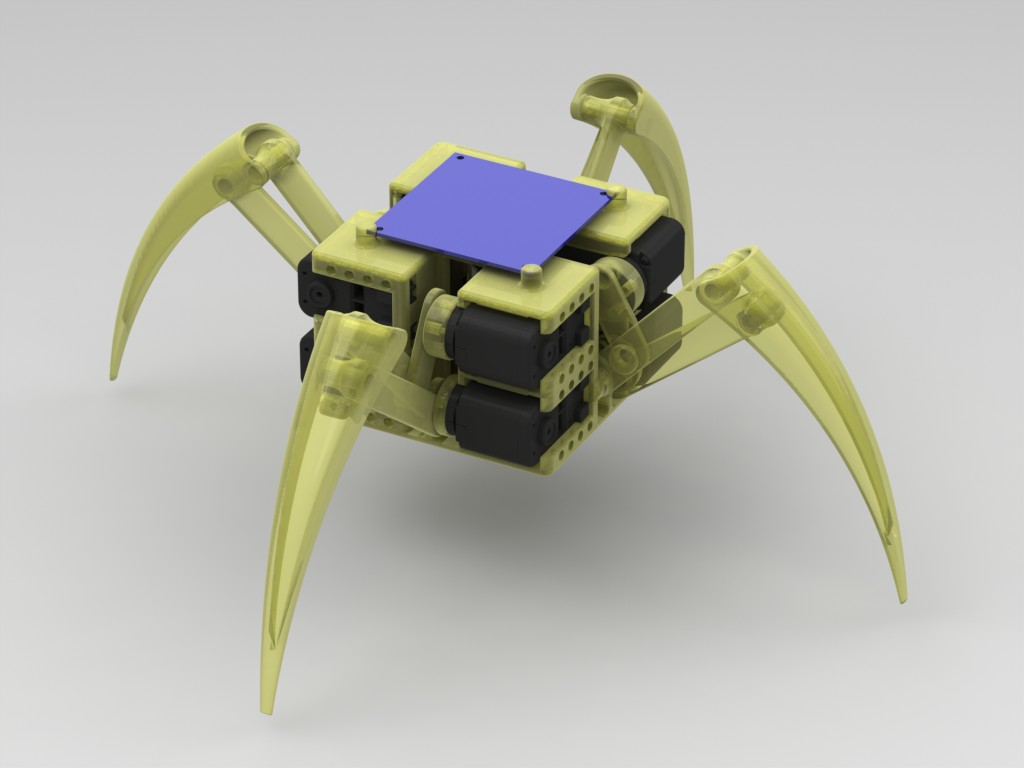
\includegraphics[width=.37\textwidth]{fig5.jpg}
\caption{Rendered CAD model of Aracna.}
\label{fi52}
\end{center}
\end{figure}



\section{Software}

The software is open-sourced Python based on the
code developed for the QuadraTot platform \citep{JY}. All code is
available on the project website \citep{WEB}. We use an infrared light
emitting diode (LED) on the robot along with an external Nintendo Wii
remote to provide feedback of the distance traveled. The robot
receives feedback from the Wii remote and internal servo sensors and
then processes the information to send the next command to
the servos. The communication between the external control computer
and the ArbotiX on-board microcontroller occurs over wireless XBee.



\section{Specifications}

\begin{figure}[t]
\begin{center}
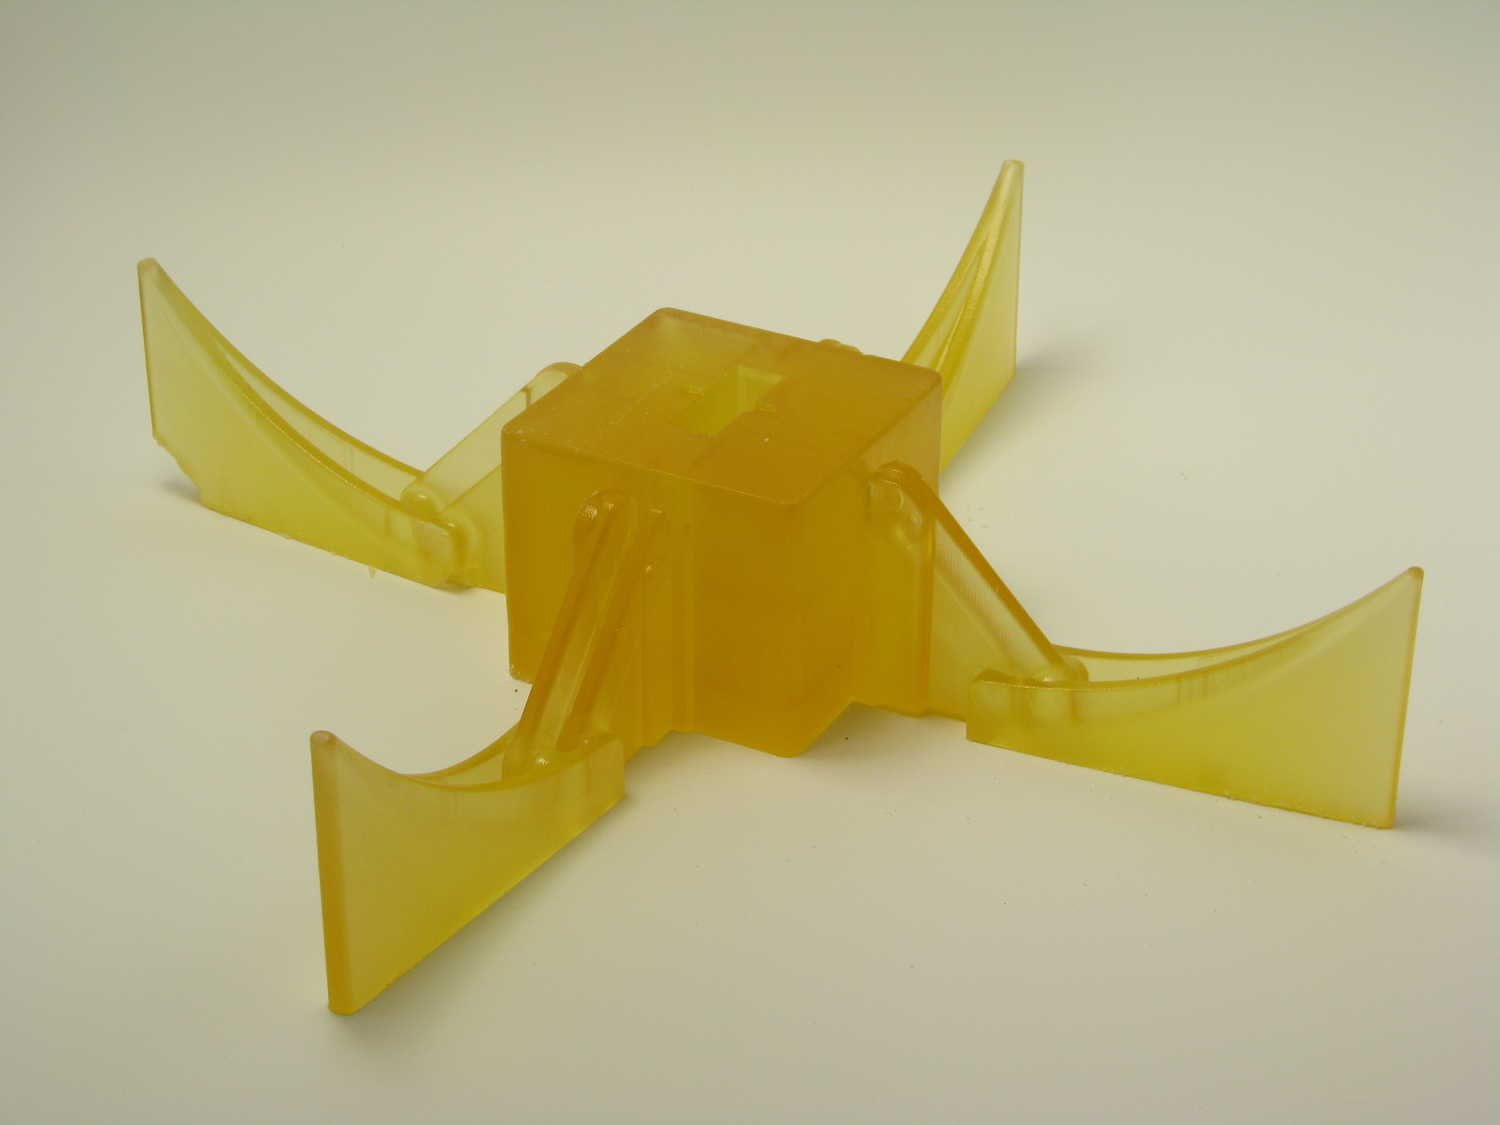
\includegraphics[width=.37\textwidth]{fig2.jpg}
\caption{Robot printed as one piece with support material intact.}
\label{fig2}
\end{center}
\end{figure}

The Aracna may be 3D printed as a single part (Figure~\ref{fig2}). On
an Object Connex500 printer, the robot was completed in 26 hours,
using approximately 1000 g of model material and 1500 g of support
material. We estimated the cost of the printed parts to be \$410 by
using an estimated model material cost of \$1/4.5g and support
material cost of \$1/8g. This cost estimate is variable depending on
the type of material used. The robot has no removable printed parts
except for the battery cover. In the near future, we will make STL files
available for printing the robot as separate parts on
3D printers with smaller tray sizes. Printing the robot as separate parts
will also reduce the amount of support material needed, and thus the
overall cost. As shown in Table~\ref{tab:cost}, the total cost of the
Aracna is just under \$1500; these estimates are based on the material
calculations above and prices from trossenrobotics.com in March 2012.

\begin{table}[h]
\center{
\begin{tabular}{|c|c|}
\hline
Part & Cost\\
\hline\hline
3D Print Materials & \$410\\
ArbotiX Robocontroller Kit & \$189\\
Dynamixel AX-18A Robot Actuator (x8) & \$721\\
3S 11.1V 2000mAh Pro Lite LiPo Battery & \$73\\
LiPo Battery Balance Charger Kit & \$70\\
Cables, Connectors, Misc & \$28\\
\hline\hline
\bf Total & \bf \$1491\\
 \hline
\end{tabular}
}
\vskip 0.25cm
\caption{Estimated total cost. A complete parts list is on our website \citep{WEB}.}
\label{tab:cost}
\end{table}



\section{Acknowledgements}

This work was supported by the National Science Foundation's Office of
Emerging Frontiers in Research and Innovation (grant number 0735953).


\footnotesize
\bibliographystyle{apalike}
\bibliography{references}
\end{document}

